\documentclass{beamer}


\graphicspath{ {pictures/} }

\usetheme{Boadilla}

\title{HLCV Project}
\subtitle{Spotting distracted drivers using classic CV methods}
\author[Reyes, Schaefer, Tonsen, Weber]{Guillermo Reyes \\
	 Daniel Schaefer \\
	 Marc Tonsen \\
 Dominik Weber\\}
 \institute[]{Saarland University}
\date{25.07.2016}



\begin{document}
	\begin{frame}
		\titlepage
	\end{frame}


    \begin{frame}{Motivation}
		\frametitle{Motivation}
        \textbf{Distraction-affected crashes 2013:}\\
        \vspace{0.5cm}
        According to U.S. Department of Transportation and the National Highway Traffic Safety Administration \cite{knuthwebsite}
		\begin{itemize}
            \item 10\% of all fatal crashes $\rightarrow$ 3.000 people killed
			\item 18\% of all injury crashes $\rightarrow$ 400.000 poeple injured
		\end{itemize}
        in motor vehicle crashes involving distracted drivers.\\
		\vspace{0.5cm}
        % these big numbers indicate a problem which has to be adressed in our opinion.
		$\Rightarrow$ Simple cameras combined with CV algorithms are non-intrusive and relatively cheap! % solution to detect distracted drivers
        % solution to detect distracted drivers compared to for example specialized sensors
	\end{frame}
	
	
	\begin{frame}
		\frametitle{Task}
		Kaggle CV Competition: State Farm Distracted Driver Detection \\
		Given a picture of the driver we have to predict the class it belongs to
		
		\begin{columns}
			\begin{column}{0.5\textwidth}
				\begin{itemize}
					\item c0: safe driving
					\item c1: texting - right
					\item c2: talking on the phone - right
					\item c3: texting - left
					\item c4: talking on the phone - left
					\item c5: operating the radio
					\item c6: drinking
					\item c7: reaching behind
					\item c8: hair and makeup
					\item c9: talking to passenger			
				\end{itemize}
			\end{column}
			\begin{column}{0.5\textwidth}  %%<--- here
				\begin{center}
					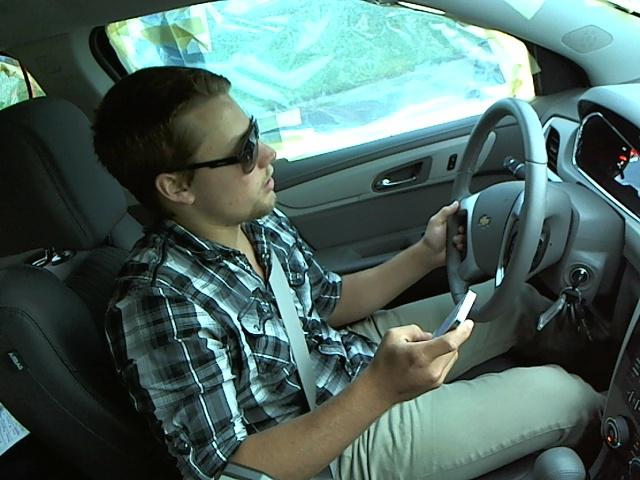
\includegraphics[width=0.9\textwidth]{img_6}
				\end{center}
			\end{column}
		\end{columns}
	\end{frame}

    \begin{frame}
		\frametitle{Classes}
			\begin{center}
                \quad drinking \quad \quad \quad \quad \quad \quad  texting left\\
				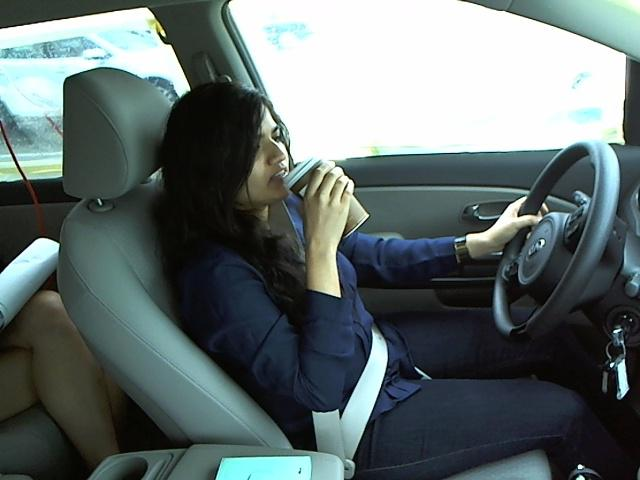
\includegraphics[width=4cm]{img_0} \vspace{0.1cm}
				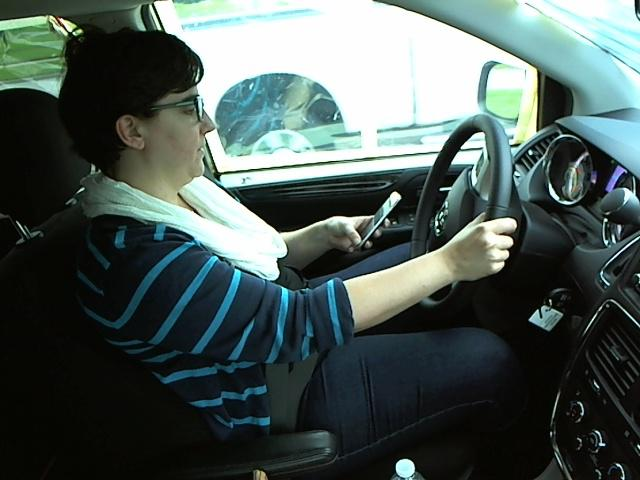
\includegraphics[width=4cm]{img_5} \\
				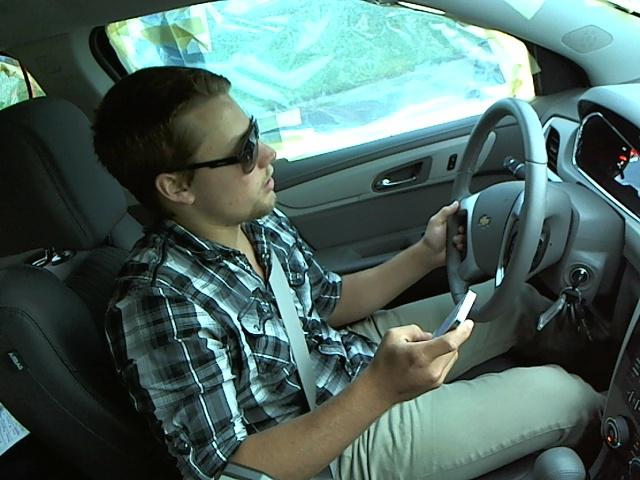
\includegraphics[width=4cm]{img_6}\vspace{0.1cm}
				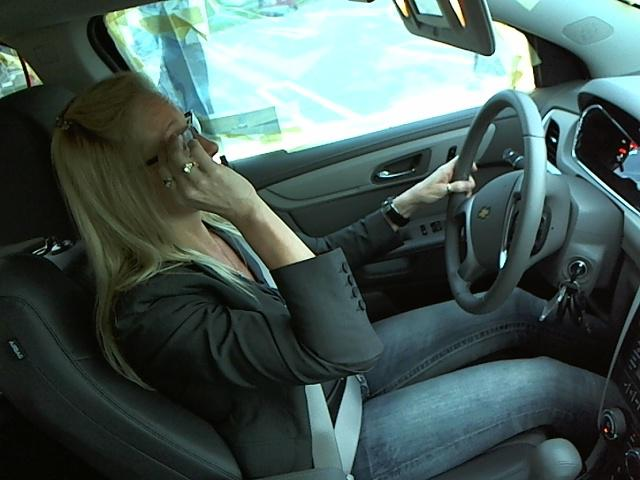
\includegraphics[width=4cm]{img_26}\\
                \quad texting right \quad \quad \quad \quad hair and makeup
			\end{center}
	\end{frame}
	
	\begin{frame}
		\frametitle{Classes}
		\begin{center}
            talking to passenger \quad \quad \quad operating radio \quad \\
			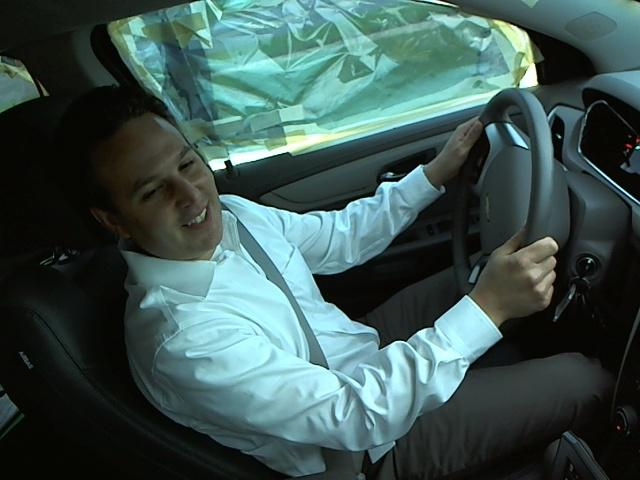
\includegraphics[width=4cm]{img_19} \vspace{0.1cm}
			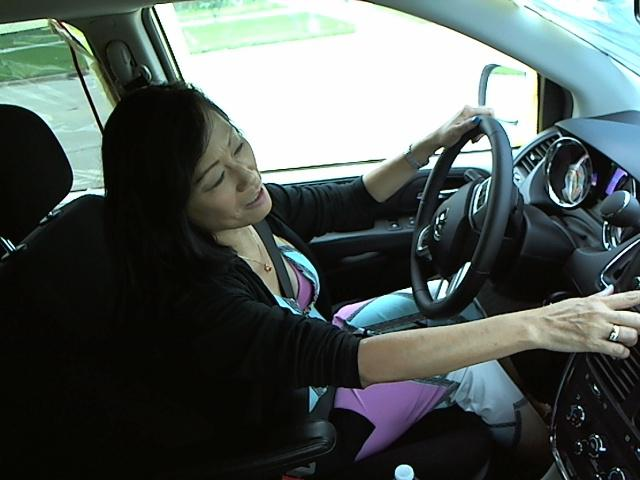
\includegraphics[width=4cm]{img_56} \\
			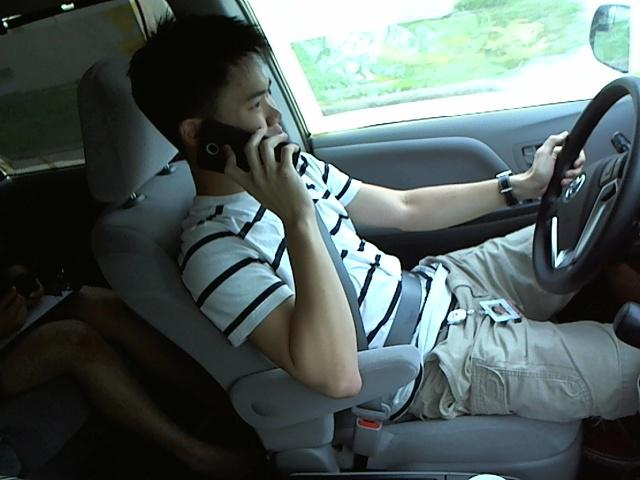
\includegraphics[width=4cm]{img_94}\vspace{0.1cm}
			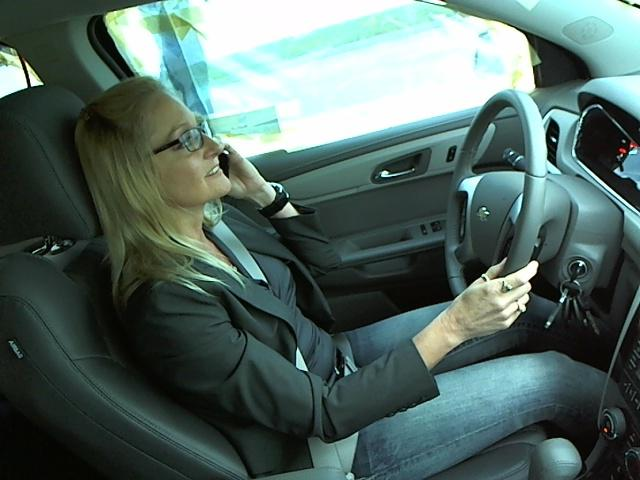
\includegraphics[width=4cm]{img_14}\\
            talking on the phone right \quad  talking on the phone left \quad \\
		\end{center}
	\end{frame}
	
	\begin{frame}
        \frametitle{Classes}
		\begin{center}
            save driving \quad \quad \quad \quad \quad \quad \quad reaching behind\\
			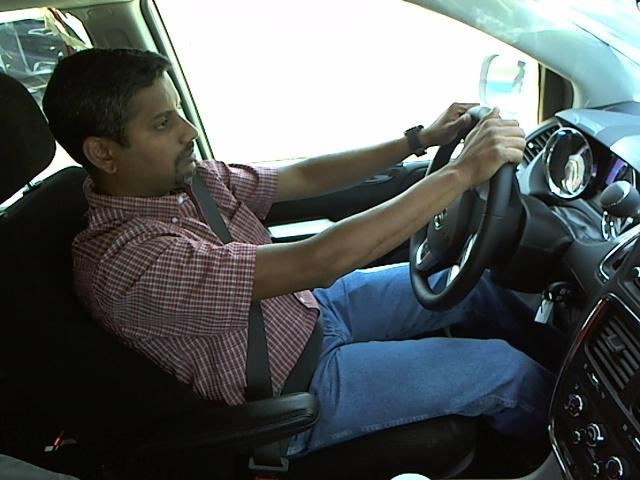
\includegraphics[width=5cm]{img_34} \vspace{0.1cm}
			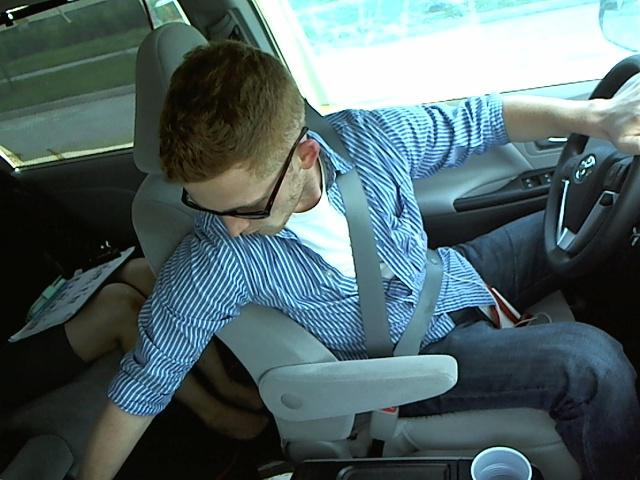
\includegraphics[width=5cm]{img_81} 
		\end{center}
	\end{frame}



    \begin{frame}{Dataset}
        \frametitle{Dataset}
        \begin{columns}
        \begin{column}{0.5\textwidth}
            \begin{itemize}
                \item 
                    around 2000 pictures per class
                    % in the available training set, which we also used for testing
                    % because we don't have the classes of the test set and we didn't
                    % want to rely on the online evaluation of the testset containing
                    % almost 80.000 pictures -> more control
                \item 
                    26 different participants
                    % with each participant having roughly the same amount of pictures
                    % per class.
                \item 
                    4 different cars (with different camera angles)
                \item 
                    different light situations
                \item 
                    sometimes very minor differences between certain classes
             \end{itemize}
        \end{column}
        \begin{column}{0.5\textwidth}
            \begin{center}
                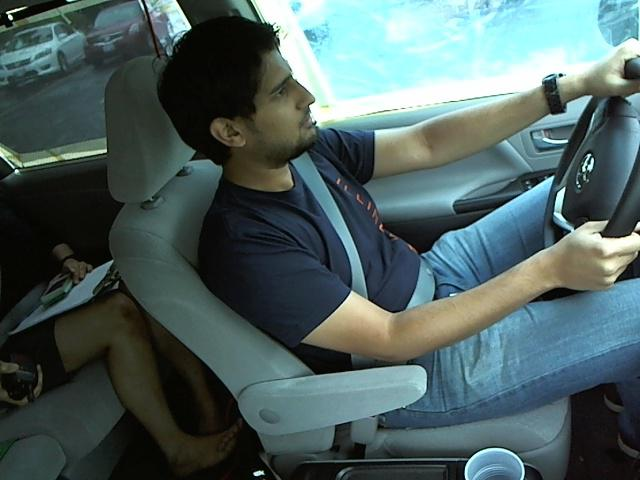
\includegraphics[width=0.8\textwidth]{c0}\\
                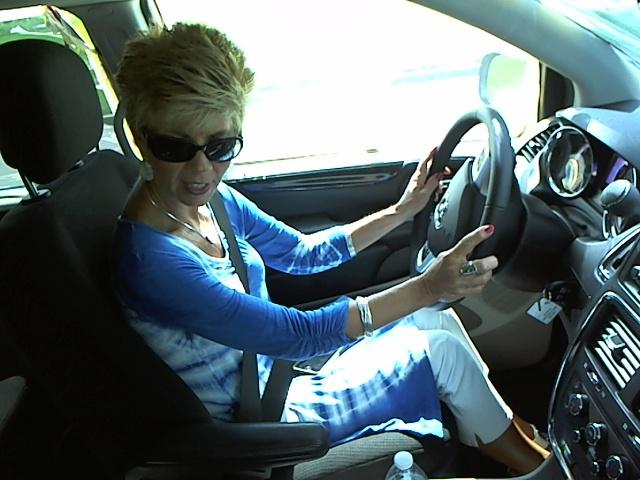
\includegraphics[width=0.8\textwidth]{c_0_angle2_passenger}
                % both of these pictures are being contained in the c0 (save driving)
                % class.
            \end{center}
        \end{column}
        \end{columns}
    \end{frame}


	\begin{frame}
		\frametitle{Related Work}
		
		\begin{columns}
			\begin{column}{0.75\textwidth}
                \textbf{Driver-Distraction Detection:}
				\begin{itemize}
					\item Datasets mostly from cameras with frontal-views, captures in artificial environments  \cite{itsc:bergasa2008}
					% \item Some approaches with specialized sensors (RGBD cameras etc.) \cite{Ragab2014}
					\item Mostly rely on gaze-tracking or head-pose estimation \cite{Dorazio} \cite{6957817}
				\end{itemize}		
                \textbf{Activity Recognition}
					\begin{itemize}
						\item Often use different sensors (e.g. wearable sensors) \cite{6258525} \cite{6365160}
						\item Camera based ones rely on continues video \cite{1315249} \cite{1430826}
					\end{itemize}	
                \vspace{0.5cm}
                $\Rightarrow$ current methods are not applicable in our case!
			\end{column}
			\begin{column}{0.25\textwidth}  %%<--- here
				\begin{center}
					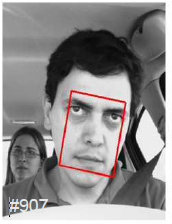
\includegraphics[width=0.9\textwidth]{frontal-view-dataset} \\
					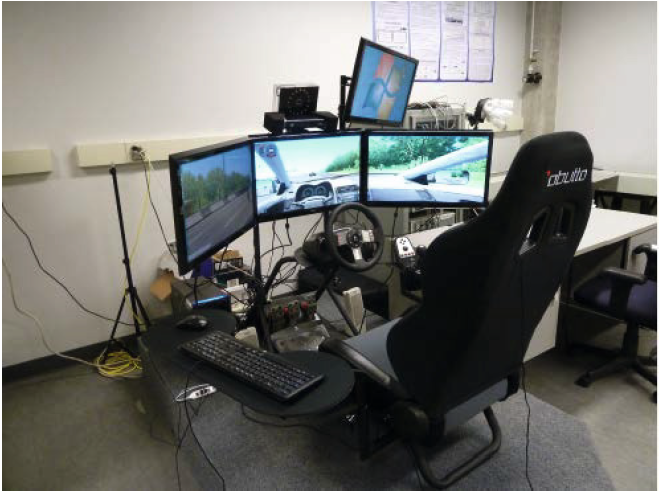
\includegraphics[width=0.9\textwidth]{RanForSim}
				\end{center}
			\end{column}
		\end{columns}
	\end{frame}
	

	\section{Approaches}

    \begin{frame}
        \frametitle{Our Approach}
        \begin{itemize}
            \item already various extremely high precision CNNs publicly available in contest-forum
            \item very limited computational ressources
            \item apply as much knowledge from the course as possible
        \end{itemize}
        \vspace{1cm}
        \begin{centering}
           \Large \textbf{$\Rightarrow$ explore possibilities of clasical computer vision}
        \end{centering}
        
    \end{frame}

	\begin{frame}
		\frametitle{Headpose-estimation}
		The Idea:
		\begin{itemize}
			\item use the headpose as a feature to predict right class
			\item narrow down the possible classes
			\item find out if picture in a specific class (ex. talking to passenger)
		\end{itemize}
	\end{frame}

	\begin{frame}
		\frametitle{Headpose-estimation}
		The Problems:
		\begin{itemize}
			\item most head-detectors didn't find a head at all caused by:
				\begin{itemize}
					\item Great variety of face-angles (frontal vs profile)
					\item Partial occlusions due to sunglasses or long hair
				\end{itemize}
			\item long computation
			\item similar classes
		\end{itemize}
		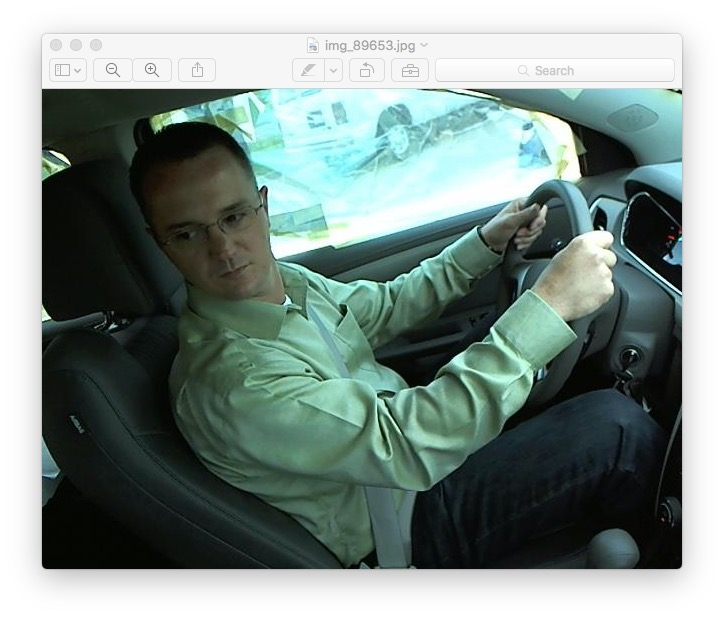
\includegraphics[width=0.45\textwidth]{img_89653} \vspace{0.1cm}
        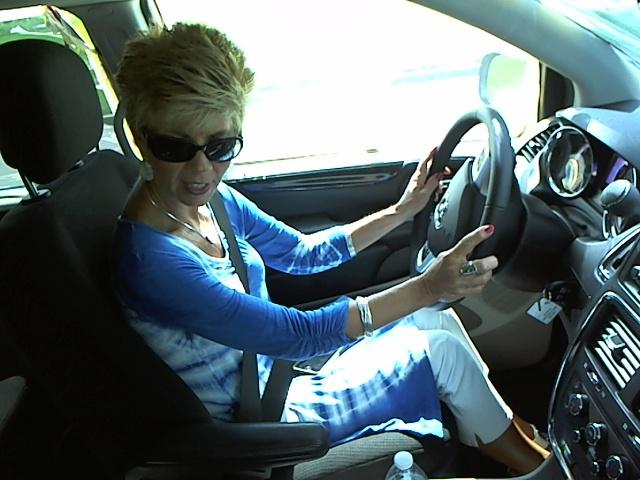
\includegraphics[width=0.45\textwidth]{c_0_angle2_passenger}
	\end{frame}

	\begin{frame}
		\frametitle{Face}
		\includegraphics[width=0.25\textwidth]{faces/face1.PNG} \vspace{0.1cm}
		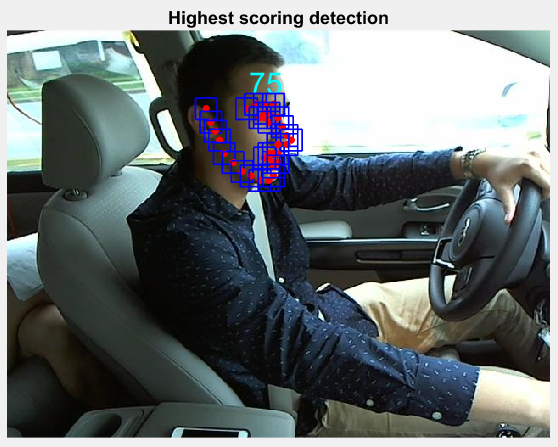
\includegraphics[width=0.25\textwidth]{faces/face2.PNG} \vspace{0.1cm}
		\begin{itemize}
			\item recognized about 75\% of the heads
			\item calculates the angle from face to camera
			\item marks 39 or 68 points in the face
			\item bad results with svm learning (insert data)
			\item recognize if talking to passenger or not (insert data)
			\item train and test with same paticipent (insert data)
		\end{itemize}
		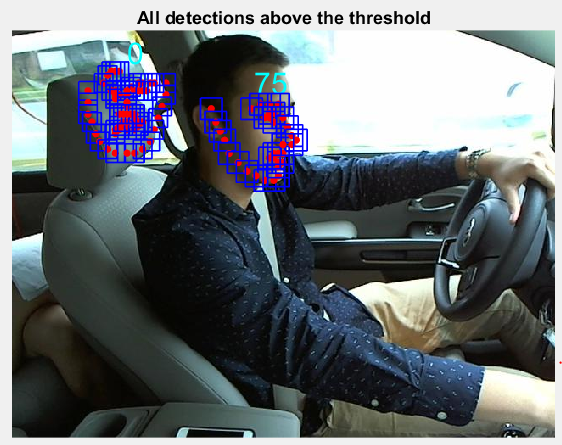
\includegraphics[width=0.25\textwidth]{faces/face3} \hspace{0.1cm}
		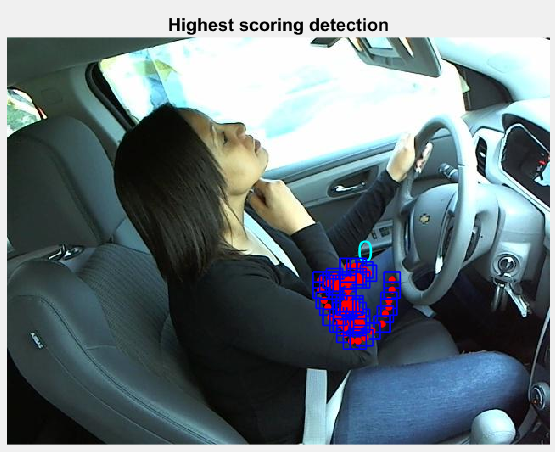
\includegraphics[width=0.25\textwidth]{faces/face7}
	\end{frame}
	
	\begin{frame}
		\frametitle{Headpose-estimation}
		Headpose distribution:
		\begin{itemize}
			\item In some cases predominant head angle is clear:		

		\end{itemize}
		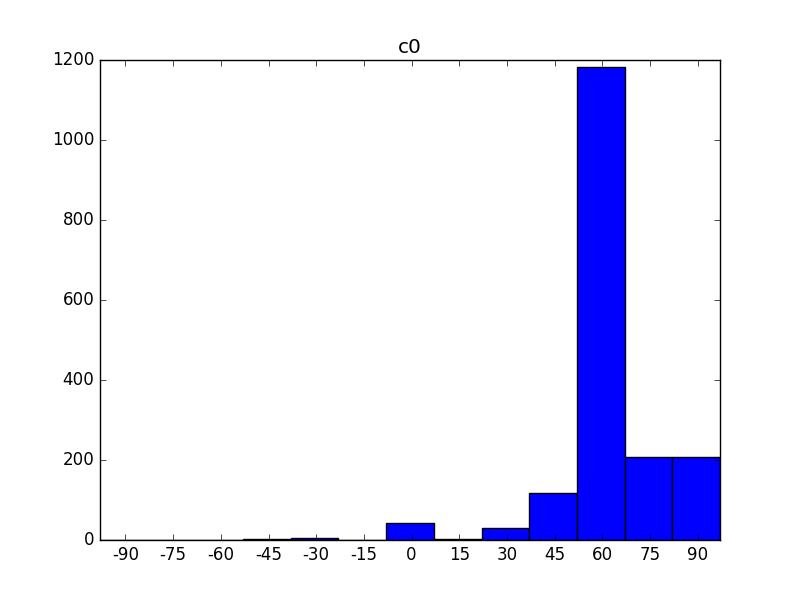
\includegraphics[width=0.5\textwidth]{headpose_evaluation_c0}
		\includegraphics[width=0.5\textwidth]{face1}
	\end{frame}
	
	\begin{frame}
		\frametitle{Headpose-estimation}
		Headpose distribution:
		\begin{itemize}
			\item In some others not that much
			

		\end{itemize}
		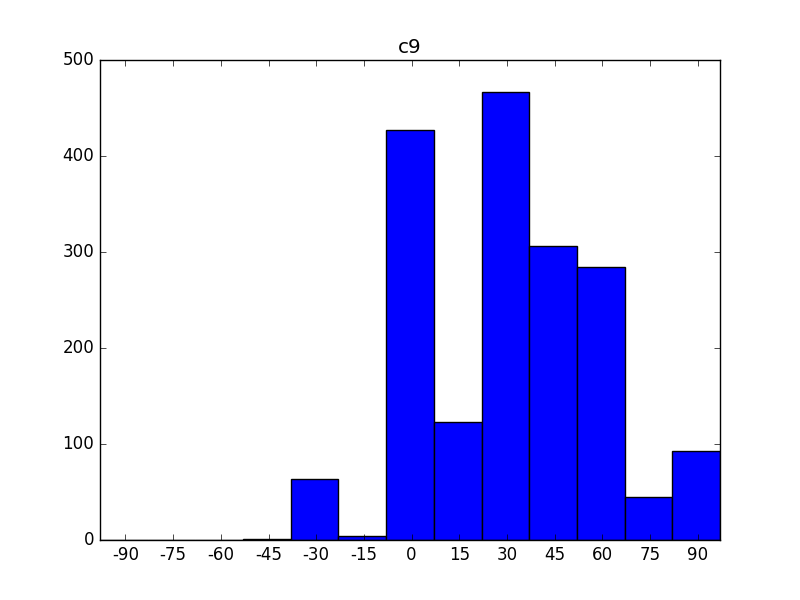
\includegraphics[width=0.5\textwidth]{headpose_evaluation_c9}
		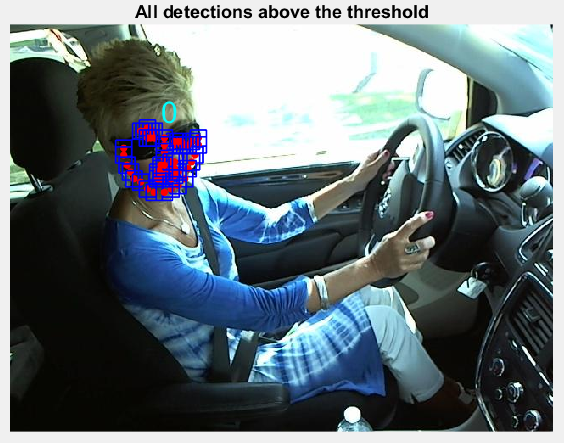
\includegraphics[width=0.5\textwidth]{face6}
	\end{frame}
	
	\begin{frame}
		\frametitle{Headpose-estimation}
		The problem with headpose:
		\begin{columns}
		 	\begin{column}{0.5\textwidth}
		 		\begin{center}
		 			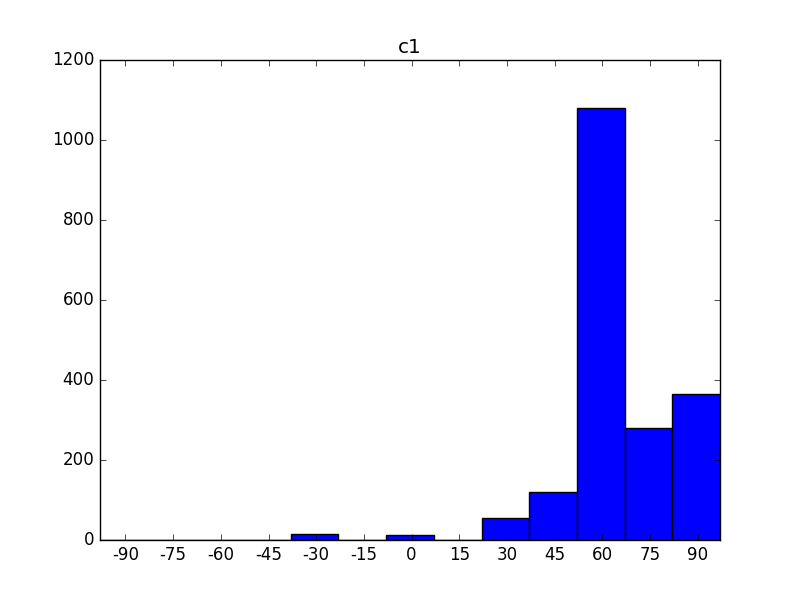
\includegraphics[width=0.85\textwidth]{headpose_evaluation_c1}\\
		 			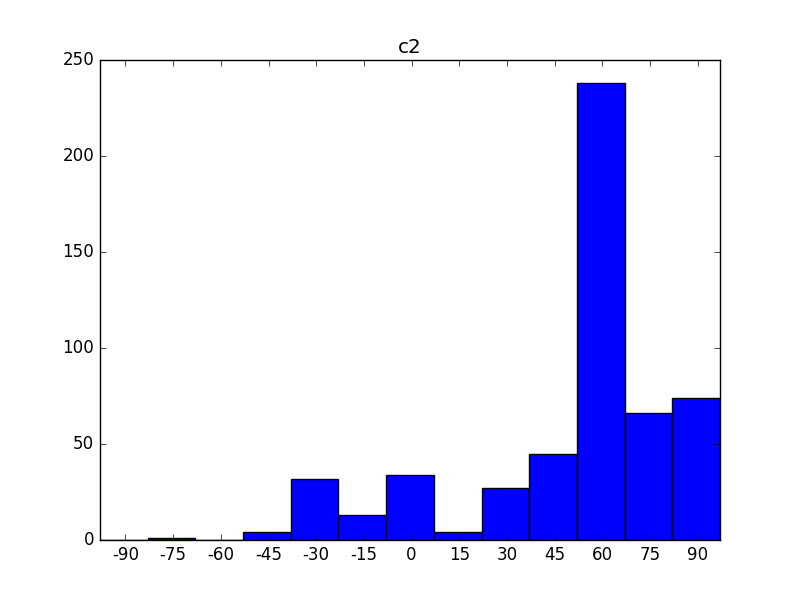
\includegraphics[width=0.85\textwidth]{headpose_evaluation_c2}
		 			% both of these pictures are being contained in the c0 (save driving)
		 			% class.
		 		\end{center}
		 	\end{column}
		 	\begin{column}{0.5\textwidth}
		 		\begin{center}
		 			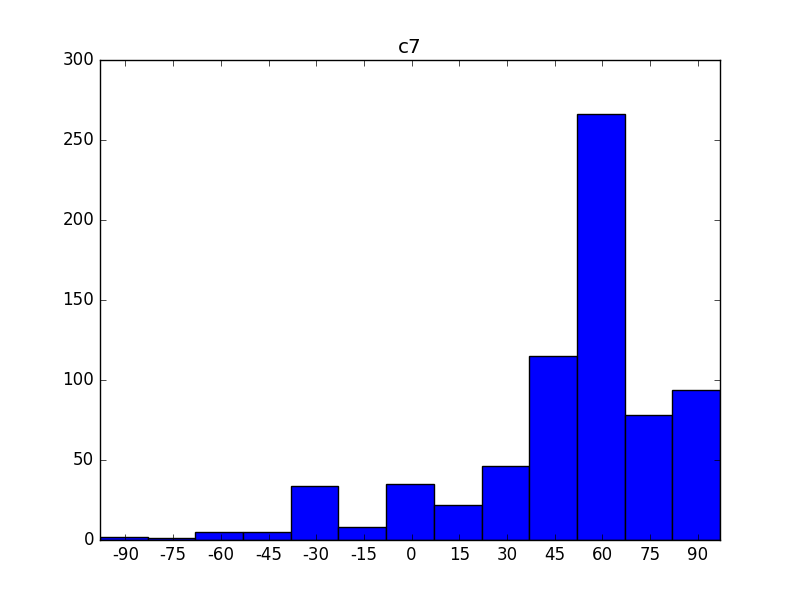
\includegraphics[width=0.85\textwidth]{headpose_evaluation_c7}\\
		 			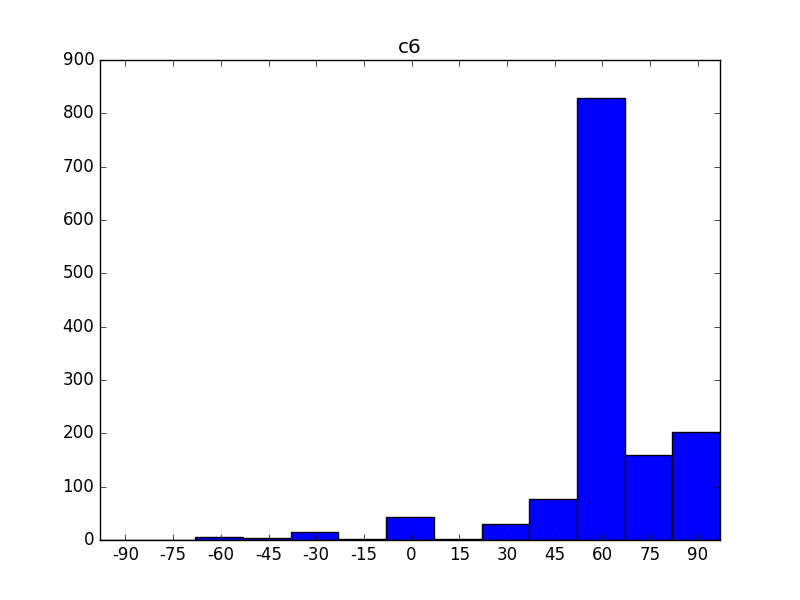
\includegraphics[width=0.85\textwidth]{headpose_evaluation_c6}
		 			% both of these pictures are being contained in the c0 (save driving)
		 			% class.
		 		\end{center}
		 	\end{column}
		 \end{columns}
		
	\end{frame}
	
	
	\begin{frame}
		\frametitle{Landmarks with HOG}		
		\begin{columns}
			\begin{column}{0.5\textwidth}
				Procedure:
				\begin{itemize}
					\item Labeled about 50 images per class with distinct class landmarks (phone, bottle, face front, face sidewards, etc)
					\item Trained a detector using HOG features for each of these landmarks
					\item To train, each of these detectors provides a boolean feature, i.e. whether the landmark is present or not
					\item Trained an SVC based on these features					
				\end{itemize}
			\end{column}
			\begin{column}{0.5\textwidth}
				\begin{center}
					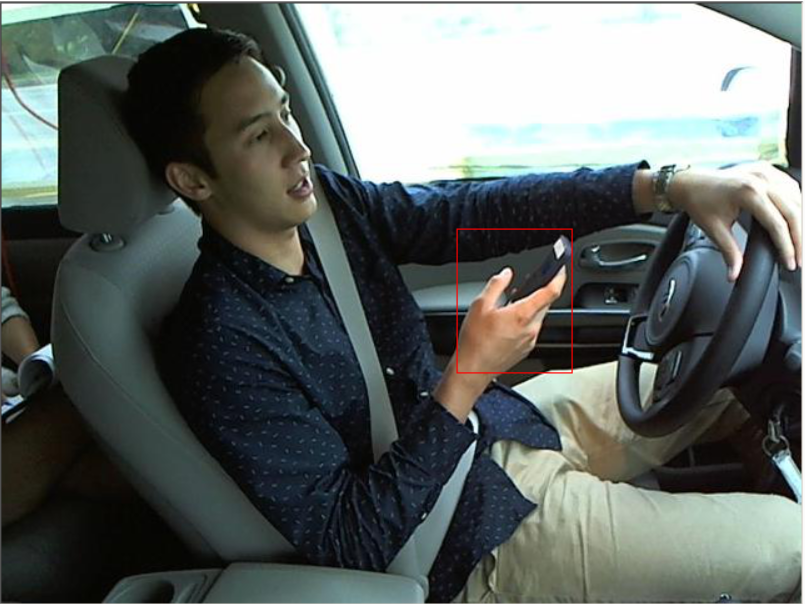
\includegraphics[width=0.85\textwidth]{mult_HOG/HOG_phone_det}\\
					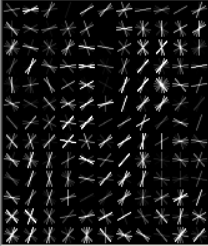
\includegraphics[width=0.5\textwidth]{mult_HOG/HOG_phone}
					% both of these pictures are being contained in the c0 (save driving)
					% class.
				\end{center}
			\end{column}
		\end{columns}
		
	\end{frame}


	\begin{frame}
		\frametitle{Landmarks with HOG: Results}
		4 Training Participants, 1 test, all classes
		\begin{columns}
			\begin{column}{0.5\textwidth}
				\begin{center}
					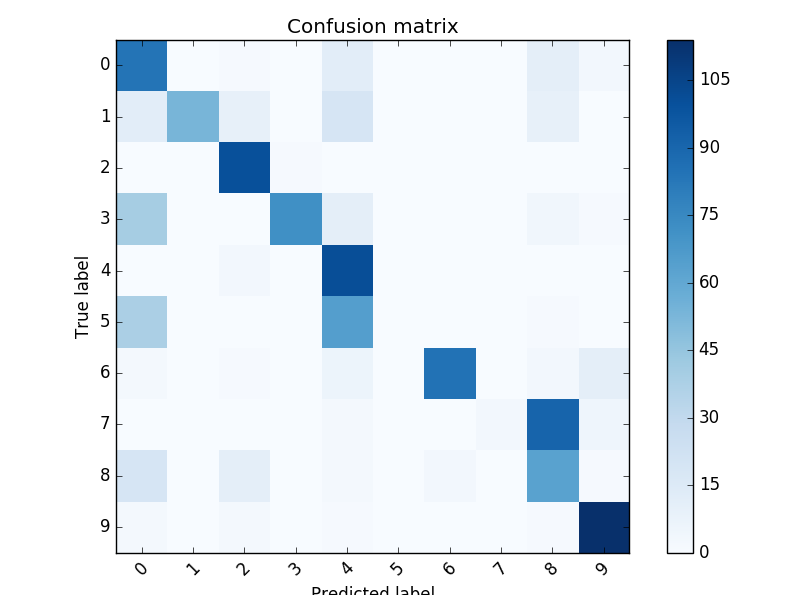
\includegraphics[width=\textwidth]{mult_HOG/4c0123456789matComparable}\\			
				\end{center}
			\end{column}
			\begin{column}{0.5\textwidth}
				\begin{center}
					%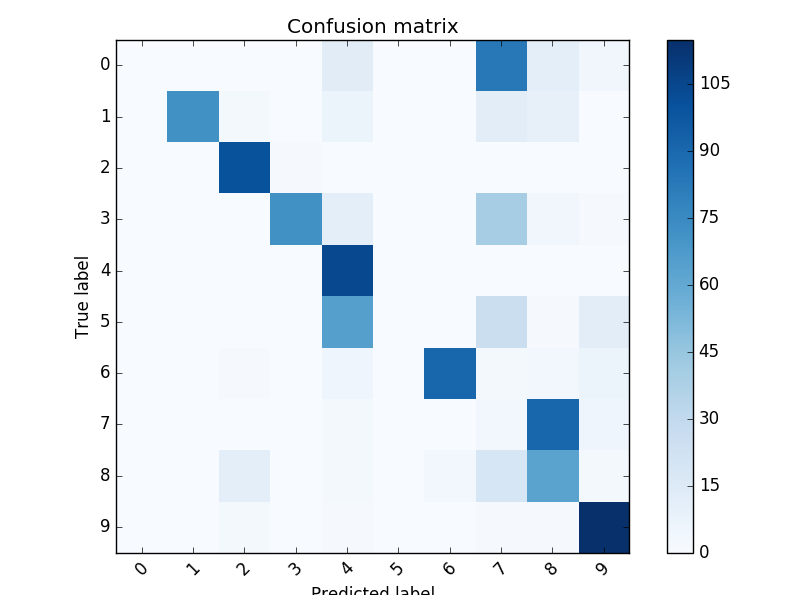
\includegraphics[width=0.85\textwidth]{mult_HOG/1c0123456789mat}\\
					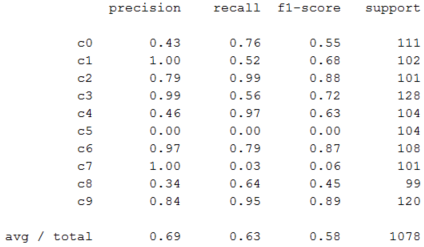
\includegraphics[width=\textwidth]{mult_HOG/4c0123456789repComparable}
				\end{center}
			\end{column}
		\end{columns}		
	\end{frame}
	
	
	
	\begin{frame}
		\frametitle{Landmarks with HOG: Results}
		4 Training Participants, 1 test, No class 7 nor 5
		\begin{columns}
			\begin{column}{0.5\textwidth}
				\begin{center}
					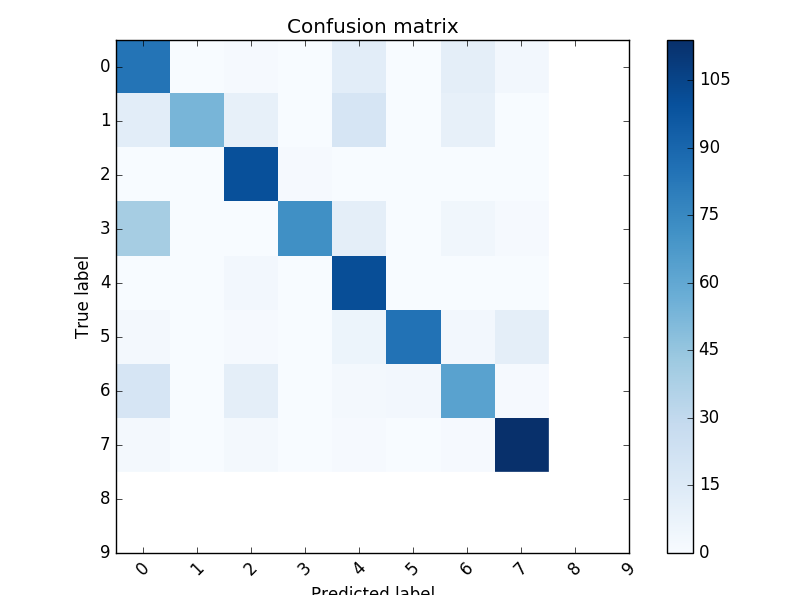
\includegraphics[width=\textwidth]{mult_HOG/4c01234689matComparable}\\			
				\end{center}
			\end{column}
			\begin{column}{0.5\textwidth}
				\begin{center}
					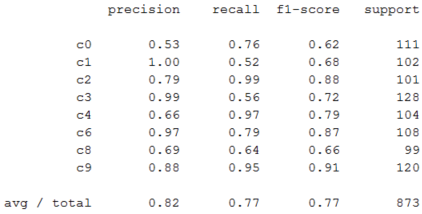
\includegraphics[width=\textwidth]{mult_HOG/4c01234689repComparable}
				\end{center}
			\end{column}
		\end{columns}		
	\end{frame}	
	
	\begin{frame}
		\frametitle{Landmarks with HOG: Results}
		4 Training Participants, several test, No class 7 nor 5
		\begin{columns}
			\begin{column}{0.5\textwidth}
				\begin{center}
					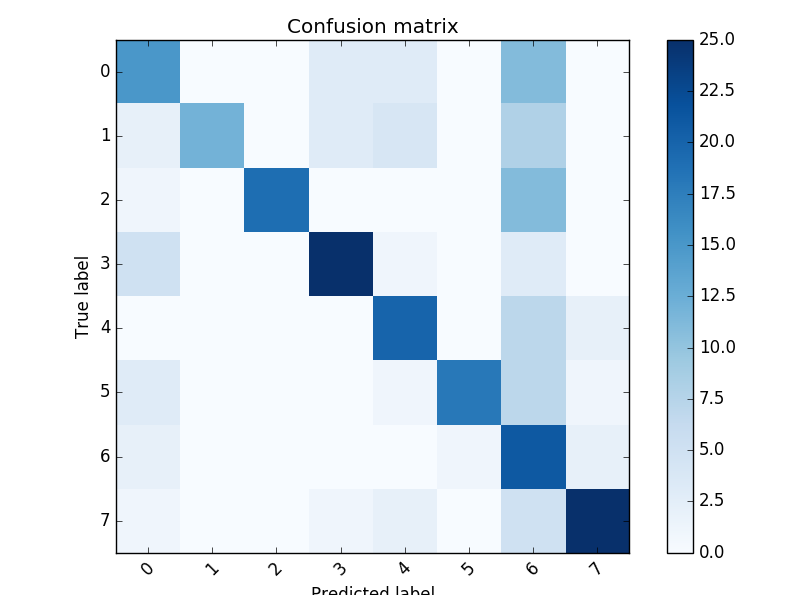
\includegraphics[width=\textwidth]{mult_HOG/4c01234689matTest2}\\			
				\end{center}
			\end{column}
			\begin{column}{0.5\textwidth}
				\begin{center}
					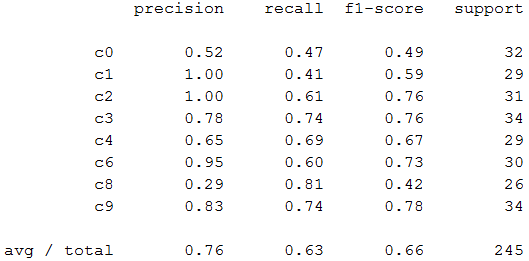
\includegraphics[width=\textwidth]{mult_HOG/4c01234689repTest2}
				\end{center}
			\end{column}
		\end{columns}		
	\end{frame}	
	
	\begin{frame}
		\frametitle{Landmarks with HOG: Improvements}		
		\begin{columns}
			\begin{column}{0.5\textwidth}
				Problems and solutions:
				\begin{itemize}
					\item Landmarks for c5(operating radio) and c7(reaching behind) Not working $\Rightarrow$ Use different ones!
					\item Landmarks for c4(Talking on phone-Left) and c8(hair and make up) produce several false positives $\Rightarrow$ make them more robust
					\item Class c0(safe driving)sometimes not very precise $\Rightarrow$ add more distinctive landmarks
				\end{itemize}
			\end{column}
			\begin{column}{0.5\textwidth}
				\begin{center}
					\includegraphics[width=0.85\textwidth]{mult_HOG/ReachingBehind}\\
					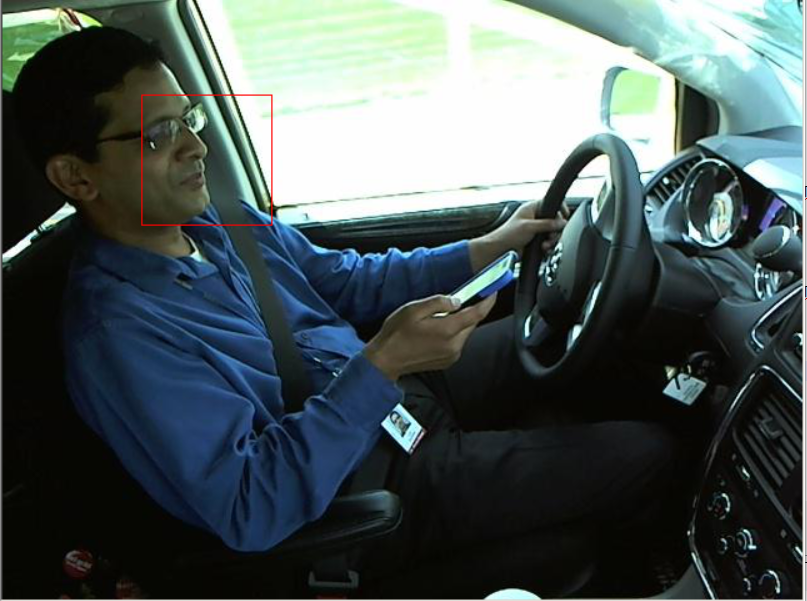
\includegraphics[width=0.85\textwidth]{mult_HOG/talk_phone_left}
				\end{center}
			\end{column}
		\end{columns}
		
	\end{frame}

    
	\begin{frame}[allowframebreaks]
		\frametitle{References} 
		\nocite{*} 
		\bibliographystyle{amsalpha} 
		\bibliography{references} 
	\end{frame}

	\medskip
\end{document}
